\documentclass{article}
\usepackage[utf8]{inputenc} %кодировка
\usepackage[T2A]{fontenc}
\usepackage[english,russian]{babel} %русификатор 
\usepackage{mathtools} 
\usepackage[left=1cm,right=1cm,top=2cm,bottom=2cm,bindingoffset=0cm]{geometry} %изменение отступов на листе
\usepackage{amsmath}
\usepackage{graphicx} 
\graphicspath{}
\DeclareGraphicsExtensions{.pdf,.png,.jpg}
\usepackage{subcaption}
\usepackage{pgfplots}
\usepackage{float}
\usepackage{graphicx}
\usepackage{hyperref}

\begin{document}
\begin{center}
    \LARGE
    Software Requirement Specification\\
    \textbf{Калькулятор посчёта бухгалтерских услуг}\\
    \LaTeX
\end{center}
\newpage

\tableofcontents
\newpage

\section{Introduction}

\subsection{Purpose}
Основная цель калькулятора бухгалтерских услуг - дать бизнесу и частным лицам 
возможность эффективно оценивать и планировать свои бухгалтерские расходы.
Это проиллюстрирует цель и полное понимания построения модели. Документ также объяснит системные ограничения и интерфейс. Этот документ предназначен для в первую очередь для заказчиков проекта, которым он будет важен для составления бизнес процессов, а также для разработчиков, так как тут описаны основные цели, которые согласованы обоими сторонами.

% \subsection{Document conventions}

\subsection{References}
https://www.rfc-editor.org/info/rfc791\\
https://www.rfc-editor.org/info/rfc793\\
https://www.w3.org/TR/html5/\\
https://www.w3.org/TR/css3-roadmap/\\
https://www.ecma-international.org/publications-and-standards/standards/ecma-262/\\
https://www.w3.org/TR/WCAG21/\\
https://www.iso.org/standard/54534.html\\

\subsection{Scope}
Документ охватывает функциональные и нефункциональные требования к веб-сайту, ориентирован на команду разработчиков, 
проектных менеджеров, и заказчика проекта. Описывает основные возможности сайта.

\section{Model Requirements FURPS+ with some attributes}

\subsection{Functional requirements}
\begin{itemize}
    \item Should have - SEC0 - Система должна предоставлять возможность авторизации пользователей с помощью имени пользователя и пароля.
    \item Should have - FR0 - Система должна поддерживать редактирование констант за услуги авторизованными пользователями.
    \item Must have - FR1 - Система должна поддреживать возможность просмотра подробного описания услуг.
    \item Must have - FR2 - Система должна поддреживать возможность добавления услуг в корзину.
    \item Must have - FR3 - Система должна поддреживать возможность удаления услуг из корзины.
    \item Must have - FR4 - Система должна поддреживать возможность просмотра количества добавленных услуг.
    \item Must have - FR5 - Система должна показывать итоговый расчёт по выбранным услугам.
    \item Could have - FR6 - Система должна предоставлять возможность заморозки услуг авторизованными пользователями.
    \item Must have - FR7 - Система должна поддреживать возможность просмотра услуг.
\end{itemize}
\subsection{Non functional requirements}
\begin{itemize} 
    \item Must have USA0 - Система должна обеспечивать адаптивный дизайн для различных устройств.
    \item Must have USA1 - Система должна обеспечивать ответ пользователю в промежутке от 200 ms до 1000 ms.
    \item Must have PERF0 - Система должна обрабатывать тысячи запросов одновременно без существенных задержек.
    \item Must have SUPP0 - Система должна легко масштабироваться для поддержки увеличения числа пользователей.
\end{itemize}

\subsection{Статусы требований}
\begin{itemize} 
    \item SEC0 - предложена
    \item FR0 - предложена
    \item FR1 - предложена
    \item FR2 - предложена
    \item FR3 - предложена
    \item FR4 - предложена
    \item FR5 - предложена
    \item FR6 - предложена
    \item FR7 - предложена
    \item USA0 - предложена
    \item USA1 - предложена
    \item PERF0 - предложена
    \item SUPP0 - предложена
\end{itemize}

\section{UML Use-Сase}
\begin{center}
    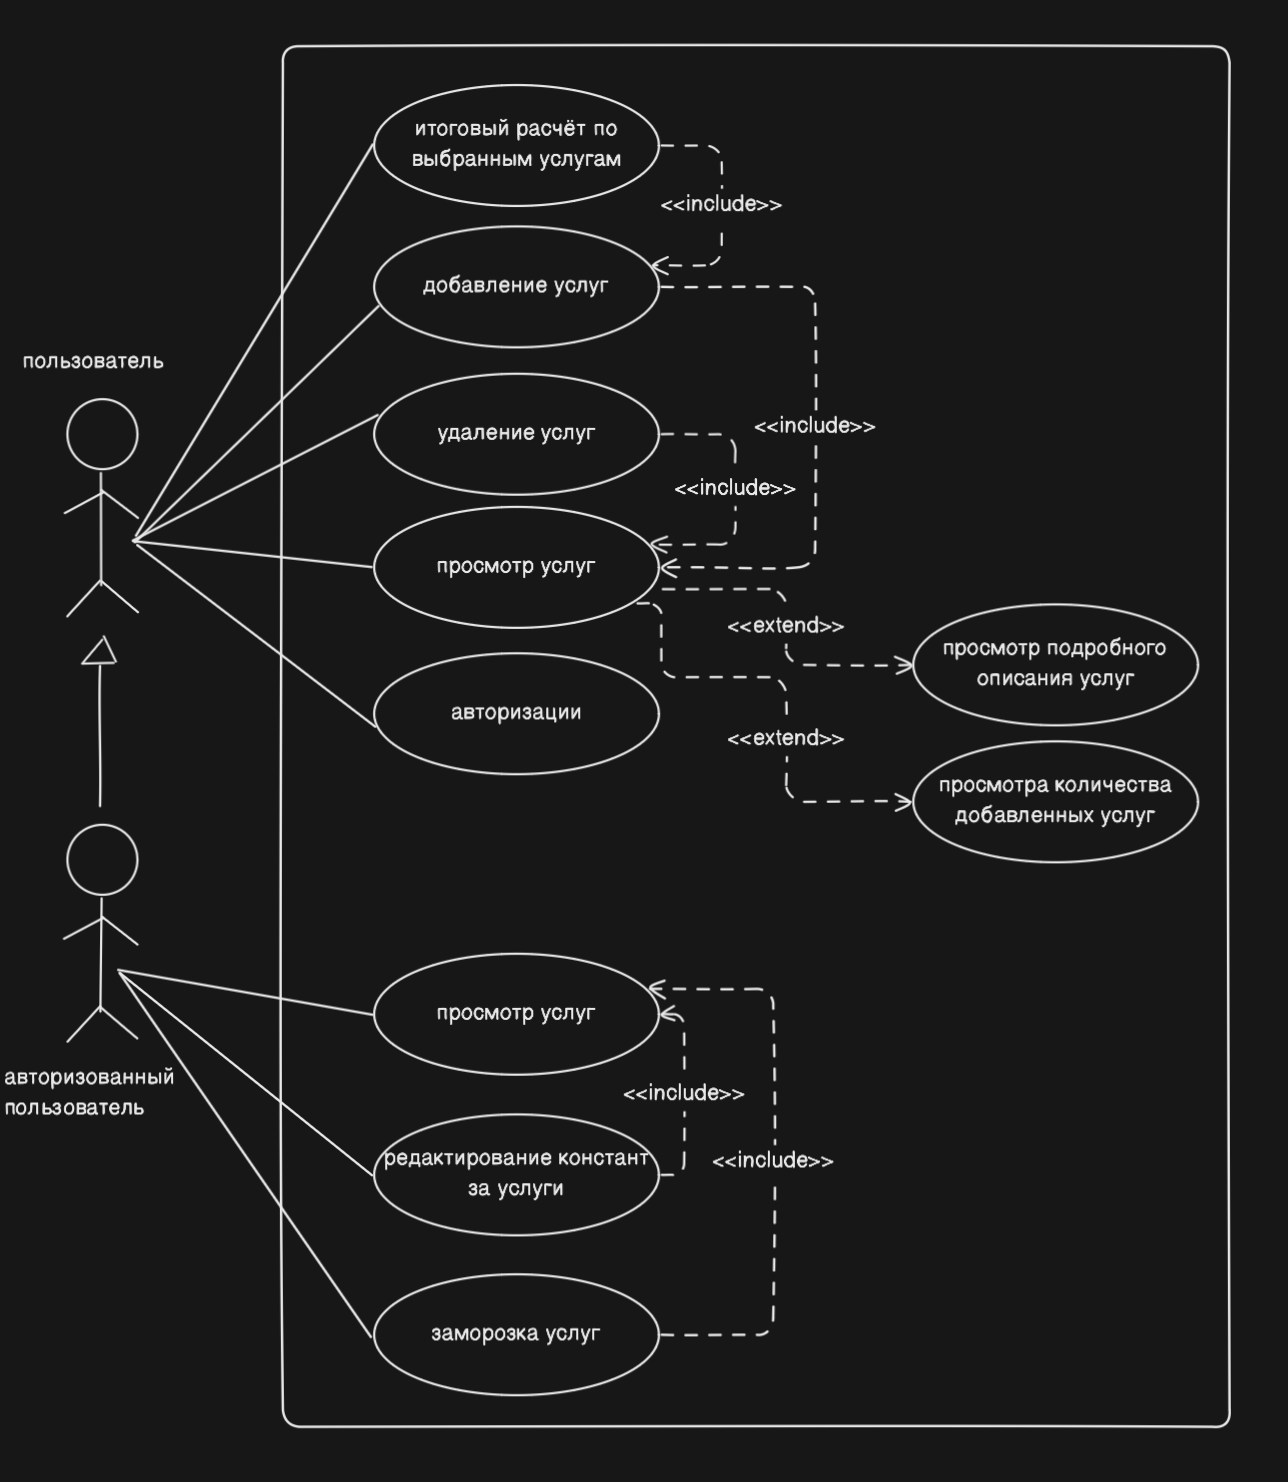
\includegraphics[width=.9\textwidth]{uml.png}
\end{center}

\section{Методология разработки}
\subsection{Waterfall}
Стандартные шаги разработки:\\
• Определение системных требований \\
• Определение требований в ПО\\
• Анализ требований\\
• Проектирование программы\\
• Разработка кода\\
• Тестирование\\
• Введение ПО в эксплуатацию\\
Есть понятие итерации между фазами разработки, есть возможность отката к предыдущей фазе. На фазе тестирования можно обнаружить, что итоговые характеристики отличаются от заданных изначально, поэтому нужно менять либо требования, либо дизайн системы.


\end{document}
\\\\\\\\\\\\\\\\\\\\\\\\\\\\\\\\\\\\\\\\\\\\\\\\\\\\\\\\\\\\\\\\\\\\\\\\\\\\\\\\\\\\\\\\\\\\\\\\\\\\\\\\\\\\\\\\\\\\\\\\\\\\\\\\\\\\\\\\\\





\includegraphics[width=.9\textwidth]{123}

\begin{verbatim}
    
\end{verbatim}

\begin{itemize}
    \item 
\end{itemize}




\section{UML: Диаграмма последовательностей.}
Это способ описания поведения системы на основе указания последовательности передаваемых сообщений.
Диаграмма состоит из вертикальных линий жизни и горизонтальных стрелок. Линии представляют отдельные объекты, а горизонтальные стрелки — сообщения и операции, передаваемые между объектами или участниками.
В диаграмме объектами выступают участники системы.
Акторы представляют пользователей или другие системы, взаимодействующие с системой, которая описывается на диаграмме. Они могут вызывать действия, которые система выполняет в ответ на их запросы.
Границы определяют внешние границы системы и представляют собой точки входа или выхода, через которые система взаимодействует с внешним миром.
Контроллеры обрабатывают запросы и управляют потоком данных в системе. Они представляют собой узлы, через которые проходят данные и управляющие выполнением операций в системе.
Сущности представляют данные и хранят состояние системы. Они могут быть представлены как базы данных или другие системы хранения данных.
Линия жизни — это вертикальная линия на диаграмме последовательности UML, которая представляет объект или участника взаимодействия и связывает его с сообщениями во времени. 
Линия жизни начинается с появления объекта на диаграмме и продолжается до его удаления или окончания взаимодействия.
